\documentclass[tikz,border=5pt]{standalone}

\usepackage{amsmath}
\usepackage{tikz}
\usetikzlibrary{arrows.meta, positioning}

\begin{document}
	
	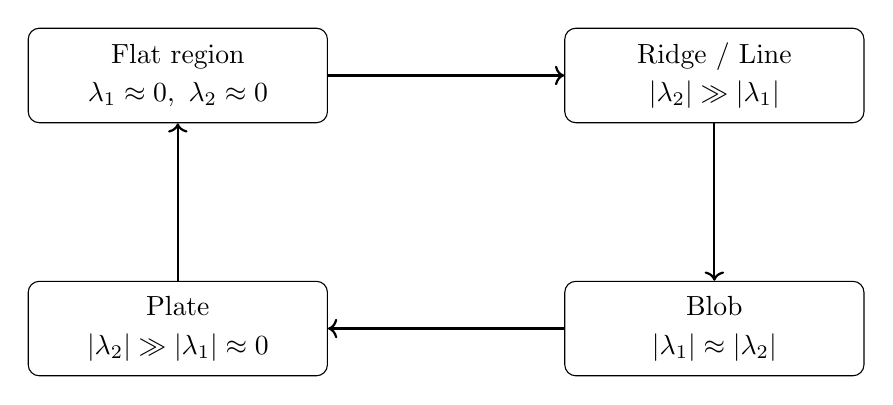
\begin{tikzpicture}[
		box/.style={draw, rounded corners, align=center, minimum width=3.8cm, minimum height=1.2cm},
		arrow/.style={->, thick}
		]
		
		% Nodes
		\node[box] (flat) {Flat region\\[2pt]
			$\lambda_1 \approx 0,\ \lambda_2 \approx 0$};
		
		\node[box, right=3cm of flat] (ridge) {Ridge / Line\\[2pt]
			$|\lambda_2| \gg |\lambda_1|$};
		
		\node[box, below=2cm of ridge] (blob) {Blob\\[2pt]
			$|\lambda_1| \approx |\lambda_2|$};
		
		\node[box, left=3cm of blob] (plate) {Plate\\[2pt]
			$|\lambda_2| \gg |\lambda_1| \approx 0$};
		
		% Arrows
		\draw[arrow] (flat) -- (ridge);
		\draw[arrow] (ridge) -- (blob);
		\draw[arrow] (blob) -- (plate);
		\draw[arrow] (plate) -- (flat);
		
	\end{tikzpicture}
	
\end{document}
